\documentclass[../Proposed Method.tex]{subfiles}
\begin{document}

% \textbf{What is GNQTS and its evolution}
Global-best guided quantum-inspired tabu search algorithm with quantum not gate (GNQTS) is a metaheuristic algorithm inspired by the superposition state of a quantum. There are three main features about GNQTS. First, after each generation, the particles will get closer and closer to the best solution. Meanwhile, keep the particles away from the wrong solutions. Second, the ability of convergence is enhanced by using the global best as a guidance. Third, quantum not gate is the key to escape local optima. With these features, GNQTS is capable of finding good solutions effectively. Figure \ref{flow} shows the flowchart of GNQTS. Algorithm \ref{GN_pseudo} is the pseudo code of GNQTS.

% \textbf{Flow chart of GNQTS}
\begin{figure}[H]
    \centering
    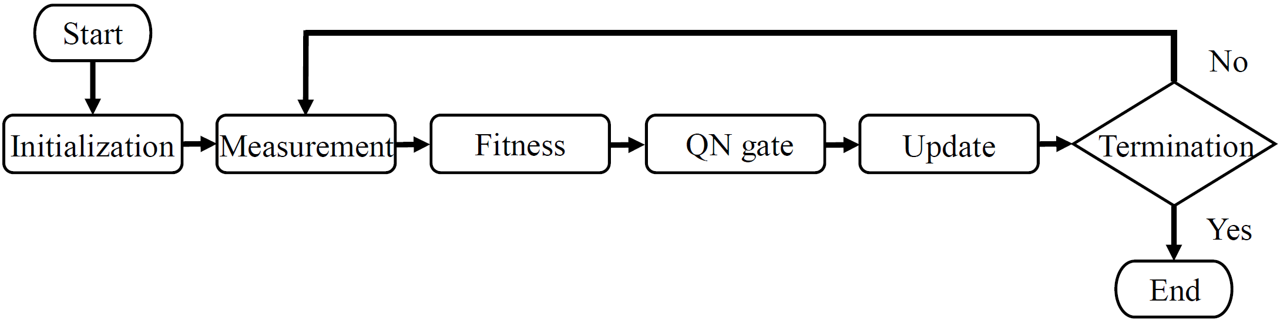
\includegraphics[scale = 0.4] {figure/flowChart.png}
    \captionsetup{font={footnotesize}}
    % \vspace{-3em}
    \caption{The flowchart of GNQTS}
    % \vspace{-0.5em}
    \label{flow}
\end{figure}

% \textbf{Pseudo code of GNQTS}
\begin{figure}[H]
    \centering
    \begin{minipage}{.6\linewidth}
        \begin{algorithm}[H]
            \caption{GNQTS}
            \label{GN_pseudo}
            \begin{algorithmic}[1]
                \State $i \leftarrow 0$
                \State Initialize quantum  population $Q(0)$
                \State Initialize best solution $b$
                \While {not termination-condition}
                \State {$i \leftarrow i + 1$}
                \State Produce neighborhood set N by measure $Q(i-1)$
                \State Evaluate $f(s)$
                \State Find the best solution $s^b$ and the worst solution $s^w$
                \State Update $b$
                \State Detect whether GNQTS is stuck in local optimal
                \If {stuck}
                \State Do Quantum Not Gate
                \EndIf
                \State Update $Q(i)$
                \EndWhile
            \end{algorithmic}
        \end{algorithm}
    \end{minipage}
\end{figure}

% \textbf{Explain each step of GNQTS}
\subsubsection{Initialztion}

In order to explore the potential of RSI and SMA, this article extends the boundary of parameters of these two indicators. We set the look-back period of RSI from 1 to 256, oversold and overbought from 0 to 100. To encode the those bits, we prepare 8 bits for the look-back period, 7 bits for the oversold and the overbought, so there are 22 bits in total. The same rule applies to SMA as well, set the look-back period of 4 parameters from 1 to 256, 8 bits for each of them, so there are 32 bits in total. After determining how many bits of RSI and SMA, we use RSI as an example the following steps.

\bigbreak

At the beginning of the algorithm, the probability of choosing each bit is stored in a array called beta matrix. Each bit in the beta matrix is set to 0.5, as in superposition state of quantum - that is, the probability of choosing 0 or 1 is 50\%. As shown in \ref{init}, where $0 \leq n \leq 21$.

\begin{figure}[H]
    \centering
    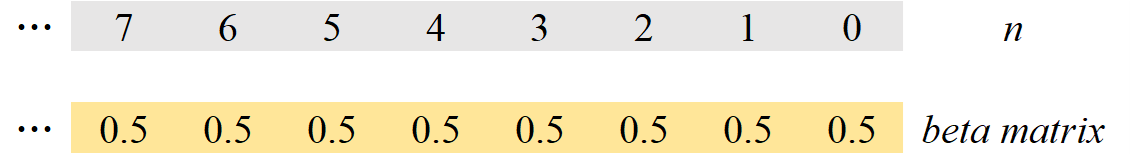
\includegraphics[scale = 0.5] {figure/init.png}
    \captionsetup{font={footnotesize}}
    \caption{Initilize beta matrix}
    \label{init}
\end{figure}

\subsubsection{Measurement}

After initializing the beta matrix, a random number $r$ is given to each bit to determine the bit should be 0 or 1, where $0 \leq r \leq 1$. Then we compare each bit with its $r$, if the probability of $bit_{n}$ in the beta matrix is greater than $r$, $bit_{n}$ is set to 1, else set to 0. The process of measurement is shown in \ref{measure}.

\bigbreak

\begin{figure}[H]
    \centering
    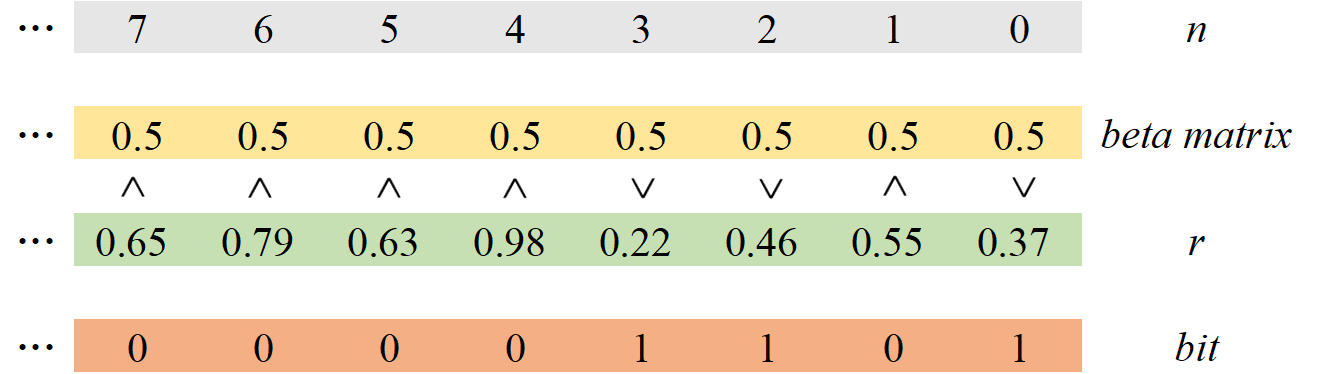
\includegraphics[scale = 0.5] {figure/measure.png}
    \captionsetup{font={footnotesize}}
    \caption{The process of forming a trading strategy in measurement}
    \label{measure}
\end{figure}

\bigbreak

After each bit is measured, we can transform these bits into decimals to form a trading strategy as shown in figur \ref{form_strategy}. In the example, 8 bits for RSI look-back period, 7 bits for the oversold and overbought. The RSI look-back period starts from 1, so add 1 to it.

\begin{figure}[H]
    \centering
    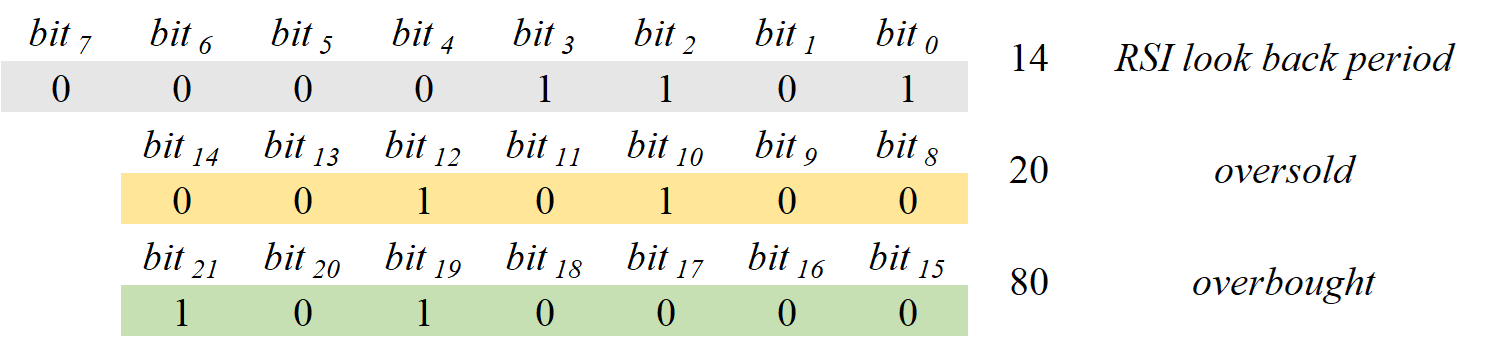
\includegraphics[scale = 0.5] {figure/form_strategy.png}
    \captionsetup{font={footnotesize}}
    \caption{An example of transform bits into trading strategy. RSI (14) (20, 80).
        RSI Look back period starts from 1.}
    \label{form_strategy}
\end{figure}

\subsubsection{Fitness}

The fitness in this paper is the rate of return. When trading strategies are generated, this paper uses simulated transactions to calculate the rate of return of each particle. The higher the rate of return is, the better is the trading strategy.

\subsubsection{Quantum Not Gate (QN Gate)}

There are three important information we need ot keep track of, which are local best particle, local worst particle and global best particle.  After calculating the rate of return in every iteration, the particle with highest rate of return is the local best, the particle with the lowest rate of return is local worst. By sorting the rate of return, it is easy to distinguish which particle is the local best and which is the local worst. We record their rate of return and trading strategy of these two particles. Then we compare the rate of return of local best and global best. If the rate of return the local best is higher than the return rate of the global best, we copy the information of local best to global best, which are strategy and rate of return. Next, according to the information of these global best and local worst, we can now execute the step of quantum not gate. First check each bit of the trading strategy of the global best and local worst.  If the global best has $bit_n = 1$, local worst has $bit_n = 0$, and $beta_n$ is below 0.5, then $beta_n = 1- beta_n$. If the global best has $bit_n = 0$, local worst has $bit_n = 1$, and $beta_n$ is over 0.5, then $beta_n = 1- beta_n$. As shown in Figure \ref{GN_gate}. We apply this rule for all 22 bits. This step makes GNQTS algoritm with the ability of escaping the local optimal.

\begin{figure}[H]
    \centering
    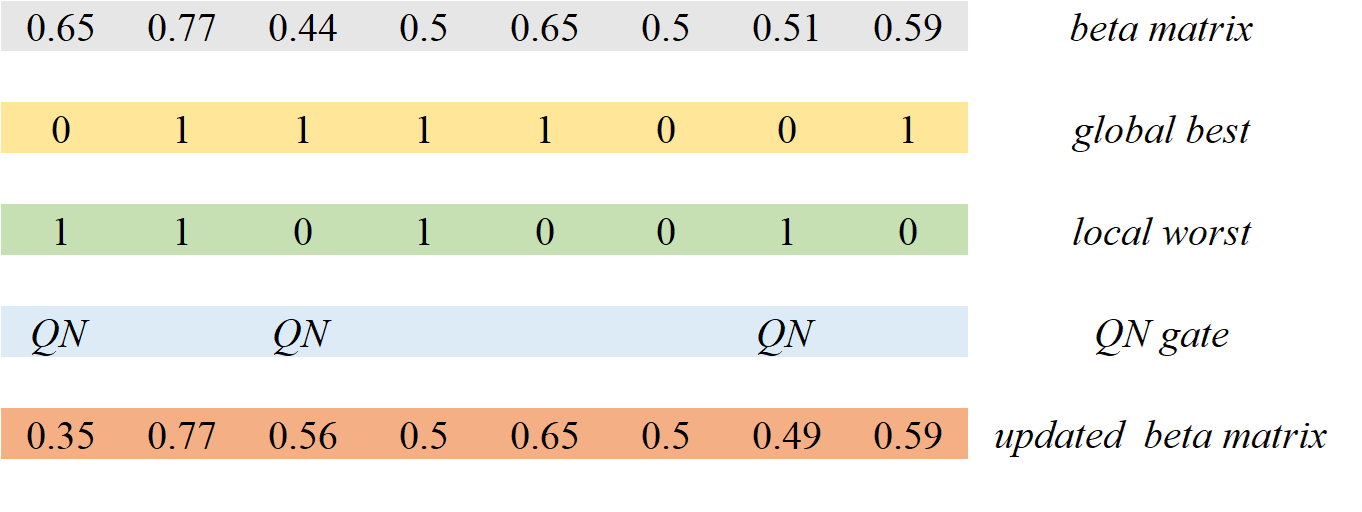
\includegraphics[scale = 0.5] {figure/GN_gate.png}
    \captionsetup{font={footnotesize}}
    \caption{The process of updating beta matrix with quantum not gate}
    \label{GN_gate}
\end{figure}

\subsubsection{Update}

Delta is used to update the beta matrix when $bit_n$ meets certain conditions. Add delta to $beta_n$ if $bit_n$ of global best is 1 and $bit_n$ of local worst is 0. Subtract delta form $beta_n$ if $bit_n$ of global best is 0 and $bit_n$ of local worst is 1. The example is shown in Figure \ref{update}.

\begin{figure}[H]
    \centering
    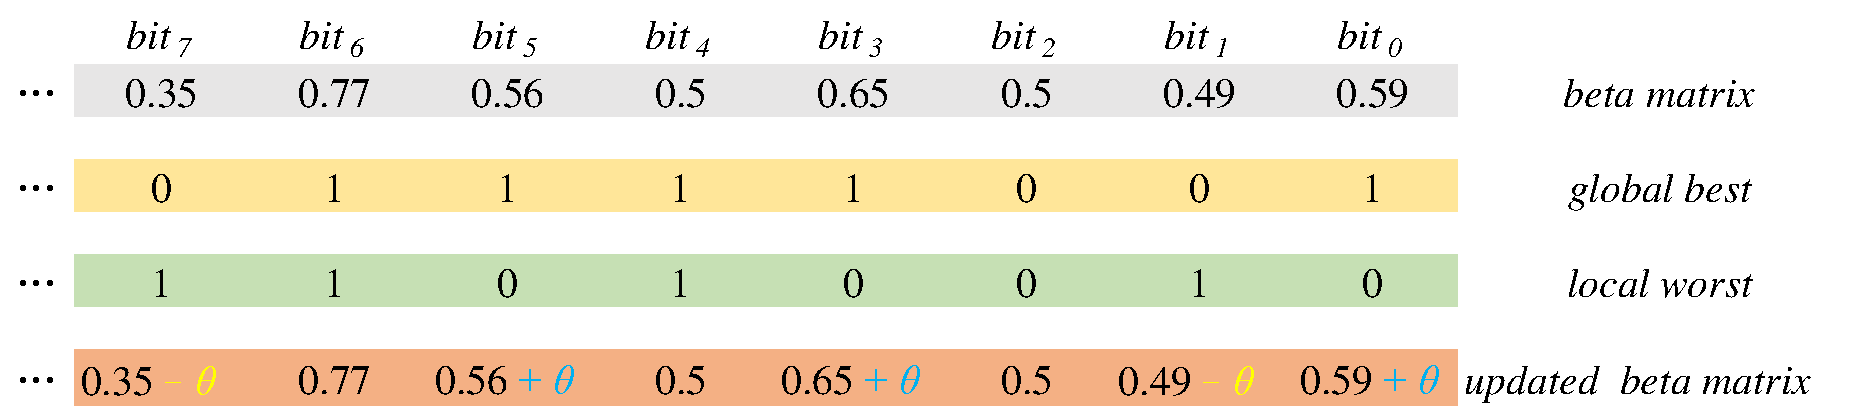
\includegraphics[scale = 0.5] {figure/update.pdf}
    \captionsetup{font={footnotesize}}
    \caption{The process of updating beta matrix with delta}
    \label{update}
\end{figure}

\subsubsection{Termination}

When the total iteration has reached or the fitness of global best is satisfied, the process of GNQTS will be terminated; otherwise, the GNQTS will will restart the loop from the measurement step.

\subsubsection{Mixing RSI and SMA}

There are two technical indicators we use in this research. Both of RSI and SMA are trained separately, in other words, either all the strategies is RSI or SMA. RSI and SMA dose not show up at the same time. To generate more flexable strategies, we proposed a method of combining RSI and SMA together while training.

\bigbreak

It is simple to use only one indicator while training. The training result uses the same indicator to form strategies, such as ($\text{RSI}_\text{buy}$, $\text{RSI}_\text{sell}$) or ($\text{MA}_\text{buy}$, $\text{MA}_\text{sell}$). If mixing two indicators together, the strategies will look like ($\text{RSI}_\text{buy}$, $\text{MA}_\text{sell}$) or ($\text{MA}_\text{buy}$, $\text{RSI}_\text{sell}$).
The proper way of implementing the beta matrix is to split the beta matrix into two part. The total bits of beta matrix will be RSI 22 bits + MA 16 bits = 38 bits. If the strategy we use is ($\text{RSI}_\text{buy}$, $\text{MA}_\text{sell}$), the first 22 bits in beta matrix belongs to RSI, the last 16 bits belongs to MA. If the strategy we use is ($\text{MA}_\text{buy}$, $\text{RSI}_\text{sell}$), the first 16 bits in beta matrix belongs to MA, the last 22 bits belongs to RSI.

\end{document}